\chapter{\chapviiiname}
\label{chapter8}




\section*{ABSTRACT}




\section{INTRODUCTION}
Development of Electrical Impedance Tomography (EIT)-based pressure sensors have hit a brick wall in the past due to the time-dependent phenomena experienced by piezoresisitive materials making them difficult to model and limiting the resistivity of such a pressure mapping sensor. This work investigates adding capacitive functionality to EIT-based pressure mapping by using a dielectric elastomer (DE) to aid capacitively shunt current so that not just the resistance of the device changes but also the capacitance. The hypothesis is that the non-linear time dependent effects of resistive sensing will be mitigated using this capacitive shunting.

As described in previous works \cite{Ellingham2024} there have been various attempts at created EIT-based pressure sensing devices. However, all of the state-of-the-art EIT-based pressure sensors rely on the change of resistance for pressure mapping \cite{,,,,}. Zhang et. al \cite{Zhang2017} utilised capacitive shunting for EIT touch mapping on a variety of surfaces with conductive coatings. Their work used a human touch input to shunt electrical current through the person's contact point, essentially mapping localised changes in capacitance. Work from Reynolds-Smith \cite{Reynoldssmith1995,Reynoldssmith1999} pioneered the bifurcation of EIT and Electric Field Tomography (EFT). 

% Dicuss differences between EIT and EFT here using Reynold-Smith theses for reference.

% fROM 	Tom Zimmerman measured the capacitance between the right hand and the left foot, and found a value of 9:1 pF [Zim95]. A simple parallel plate model of feet in shoes with 1cm thick soles gives a capacitance of 35 nF, using C = 0A=d, and taking A = 2 feet 20cm  10cm and d = 1cm. For 10 cm thick platform shoes, the value of C = 3:5nF. (We have neglected the dielectric constant of the soles, and all inductive eects.)

The lack of control over the object being shunted through makes pressure mapping estimates non-trivial.

To create a sensing domain that can map loads and estimate the corresponding pressure using this shunting phenomena three main components have been used. A conductive particle elastomer composite (CPEC) top layer, an insulating dielectric elastomer (DE) middle layer, and a grounded conductive bottom layer, as shown in Figure \ref{fig:DE-EIT_cap_shunt}. The top layer has 16 boundary electrodes connected for use with EIT drive circuitry. The bottom layer is connected to the EIT drive circuitry's ground via a singular electrode. This bottom surface will be used to shunt the current capacitively, with localised changes in capacitance due to loading causing localised changes in shunting of current.

\begin{figure}[H]
	\centering
	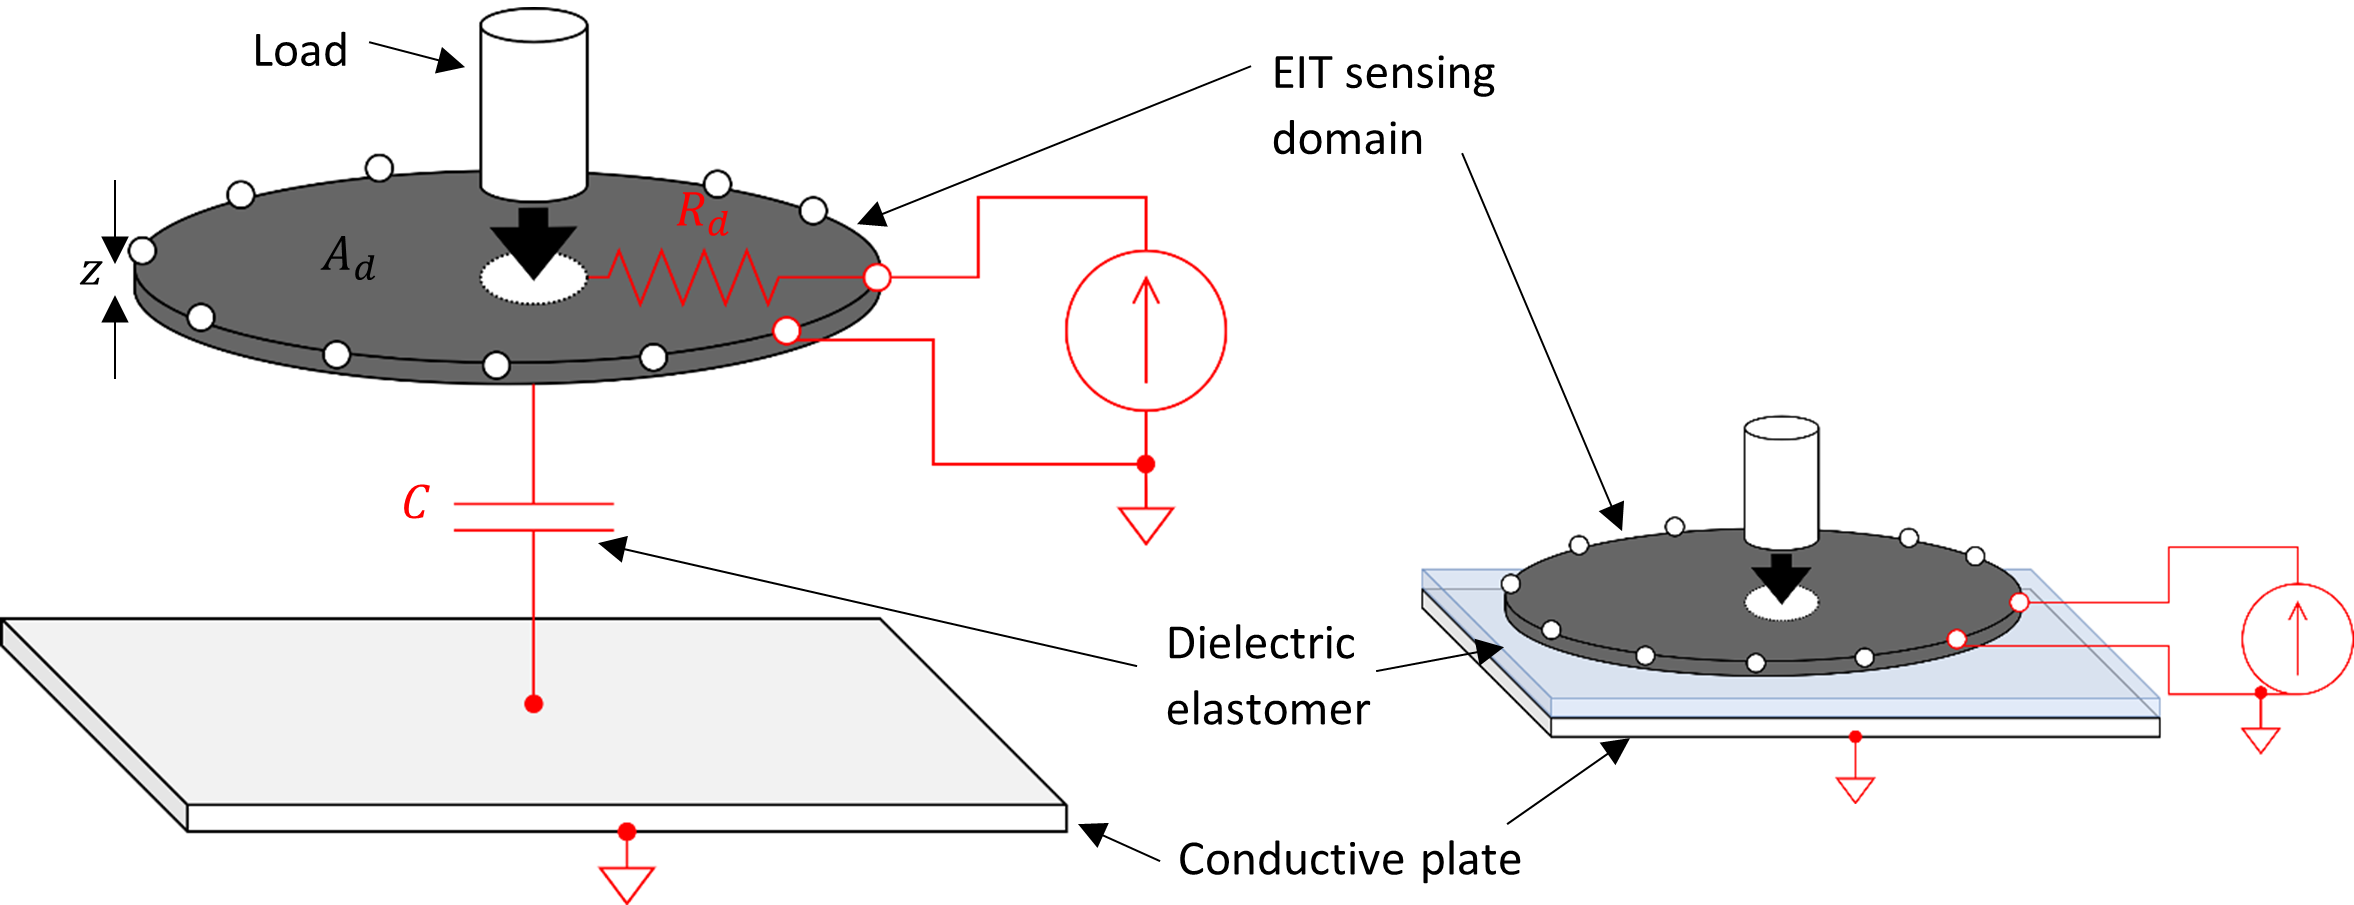
\includegraphics[width=0.9\linewidth]{Figures/cap-shunt-draft.png} % Todo: change the diagram 
	\vspace{0.3cm}
	\caption{Capacitive shunting experimental system architecture}
	\label{fig:DE-EIT_cap_shunt}
\end{figure}

% Add how this works in terms of input to the EIT algorithm. i.e. essentially we're still treating it as a purely resistive domain and hoping that the localised change in impedance (i.e. resistance and capacitance) will be mapped.

This work investigates whether the EIT drive frequency can be optimised for an EIT-based pressure sensor with range of DE shapes and thicknesses.


\section{METHOD}
% Iterate through frequencies to get various plots for power loss using the above tutorial template. This same process can be replicated for a range of different DEA shapes and DE thicknesses. Then we can show an 'optimal' frequency for gathering data from each sample then compare that with the results gathered from the EIT reconstructions.

% grab content produced for Johannes Mersch as experimental instructions explaining the theory.

% See 'Frequency domain modeling of a capacitor' from COMSOL (models.acdc.capacitor_ac.pdf)


\section{RESULTS}




\section{DISCUSSION}




\section{CONCLUSIONS}

%\afterpage{\blankpage}